\begin{frame}
  \frametitle{Overview of my MSc Dissertation}
  \begin{itemize}
  \item In BI, estimating the posterior is the major difficult task
  \item Remember, \( posterior \propto likelihood * prior \)
  \item When the likelihood is intractable \( \rightarrow\) Likelihood-free inference (LFI) methods
  \item That was my MSc about:
    \begin{itemize}
    \item Extending ROMC, a likelihood-free inference method
    \item Initial paper by~\cite{Ikonomov2020RobustOM}
    \item Implementing ROMC ELFI, a python package for LFI
    \item \href{https://elfi.readthedocs.io/en/latest/}{https://elfi.readthedocs.io/en/latest/}    \end{itemize}
  \end{itemize}

  \noindent\makebox[\linewidth]{\rule{\paperwidth}{0.4pt}}
  LFI methods approximate the posterior when the likelihood is intractable - \alert{very difficult problem}
\end{frame}

\subsection{Likelihood-free inference methods}

\begin{frame}
  \frametitle{Cases of intractable likelihood}
  \begin{itemize}
    \item What causes an intractable likelihood?
    \begin{itemize}
    \item Many reasons (e.g. intractable partition functions in unnormalized statistical models)
    \item Most common reason \( \rightarrow \) \alert{unobserved/latent variables}
    \item Latent variables are really important in many modelling cases (example in next slide)
    \end{itemize}
  \item Simulator-based models (those with intractable likelihood) are widely-used in natural sciences i.e. biology, epidemiology, neuroscience
    \item An overview of the field in \cite{Cranmer30055}

    \end{itemize}
\noindent\makebox[\linewidth]{\rule{\paperwidth}{0.4pt}}
Simulator-based models provide valuable \alert{modelling freedom}
\end{frame}

\begin{frame}
  \frametitle{Example of intractable likelihood (1)}
\begin{itemize}
  \item Predict the grade $y$ of a candidate at an important test
  \item Grade is a direct consequence of two things
  \begin{itemize}
    \item $u_1 \in [0,10]$ the mental readiness of the candidate
    \item $u_2 \in [0,10]$ the knowledge of the topic
  \end{itemize}
\item the mental readiness is direct consequence of
  \begin{itemize}
  \item $x_1$ how many hours he has slept the previous night
  \item $x_2$ how many times he has been in stressful exams in the past
  \end{itemize}
\item knowledge of the topic
  \begin{itemize}
  \item $x_3$, years of experience in software engineering
  \item $x_4$, number of application he has developed
  \end{itemize}
\end{itemize}
  \noindent\makebox[\linewidth]{\rule{\paperwidth}{0.4pt}}
  Think more about it; \alert{it is sensible to model the latent variables!}
\end{frame}


\begin{frame}
  \frametitle{Example of intractable likelihood (2)}
  \begin{itemize}
    \item \( L(\thetab) = p(D|\thetab) \propto \prod_i^N p(y^i|x^i, \thetab) = \int_{u_1,u_2}p(y^i, u^i|x^i, \thetab) \)
    \item The likelihood is defined over an integral - intractable in the general case
    \item But sampling is feasible i.e. draw \( y \sim p(y|x, \thetab) \)
  \end{itemize}

  \begin{figure}[!h]
  \tikzstyle{observable} = [draw, circle, minimum size=.6cm, inner sep=0pt,
    fill=black!30!green]
  \tikzstyle{latent} = [draw, circle, minimum size=.6cm, inner sep=0pt]
  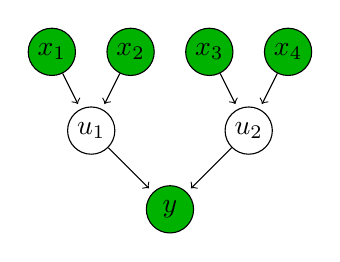
\begin{tikzpicture}[scale=.3]
  \node (x1) [observable, xshift=0cm]{$x_1$};
  \node (x2) [observable, xshift=0cm, right of=x1] {$x_2$};
  \node (x3) [observable, xshift=0cm, right of=x2] {$x_3$};
  \node (x4) [observable, xshift=0cm, right of=x3] {$x_4$};
  \node (u1) [latent, xshift=-.5cm, below of=x2] {$u_1$};
  \node (u2) [latent, xshift=.5cm, below of=x3] {$u_2$};
  \node (y) [observable, xshift=1cm, below of=u1] {$y$};

  \draw [->, shorten >=2pt] (x1) -- (u1);
  \draw [->, shorten >=2pt] (x2) -- (u1);
  \draw [->, shorten >=2pt] (x3) -- (u2);
  \draw [->, shorten >=2pt] (x4) -- (u2);
  \draw [->, shorten >=2pt] (u1) -- (y);
  \draw [->, shorten >=2pt] (u2) -- (y);
  \end{tikzpicture}
\end{figure}

\noindent\makebox[\linewidth]{\rule{\paperwidth}{0.4pt}}
If we want latent variables, we \alert{have to use likelihood-free methods.}

\end{frame}

\subsection{Robust Optimization Monte Carlo (ROMC)}

\begin{frame}
  \frametitle{Optimization Monte Carlo (OMC)}
  \begin{itemize}
    \item Core idea: \alert{Convert random sampling to a deterministic process} \cite{NIPS2015_a284df11}
      \begin{equation}
        x \sim p(x|\thetab) \Rightarrow f(\thetab, v) \rightarrow x
      \end{equation}

      \item $v$ is the nuisance variable that absorbs all the randomness
      \item $\argmax_{\thetab} p(x=x_0|\thetab) \rightarrow \argmin_{\thetab}|f(\thetab, v=v_0) - x_0| $
      \item In a computer program, the value that governs all randomness is the random seed
  \end{itemize}

  \noindent\makebox[\linewidth]{\rule{\paperwidth}{0.4pt}}
  Maximizing the probability of generating some data can be converted to a \alert{deterministic optimization process}
\end{frame}

\begin{frame}
  \frametitle{Robust Optimization Monte Carlo (ROMC), step (1)}
  \begin{itemize}
  \item What is the objective? A way to approximate the intractable $L(\thetab)=p(D|\thetab)$
  \item What I have? Only a way to simulate points from
    $p(y|\xb, \thetab)$ (random simulator)
  \item Draw random seeds $s$ and generate deterministic simulators $f_i(\thetab)$
  \item For every $f_i$, search for the
    $\thetab_i^* = argmin_{\thetab} |f_i(\thetab) - D|$
  \item For every $f_i$, define an area $\mathcal{S}_i$ around
    $\thetab_i^*$ such that $|f_i(\thetab) - D| < \epsilon$
  \item $\mathcal{S}_i$ is the acceptance region of the $i-th$ simulator
  \end{itemize}

  \noindent\makebox[\linewidth]{\rule{\paperwidth}{0.4pt}}
  Convert random sampling to an optimization process and find the parameters $\thetab_i$ that generate data close to the observations.

\end{frame}

\begin{frame}
  \frametitle{Robust Optimization Monte Carlo (ROMC), step (2)}
  \begin{itemize}
  \item The approximate posterior is the sum of all such regions $S_i$, scaled by the prior
    \begin{equation}
      p(\thetab|D) \approx p(\thetab) \frac{1}{N} \sum_i \mathcal{S}_i(\thetab)
    \end{equation}
    where $\mathcal{S}_i(\thetab) = \frac{1}{V}$ if $|f_i(\thetab) - D| < \epsilon$, otherwise $0$
  \item Each point inside the area is equally probable to have generated the data
  \end{itemize}

  \noindent\makebox[\linewidth]{\rule{\paperwidth}{0.4pt}}
  The posterior approximation is the sum of all the regions $\mathcal{S}_i(\thetab)$ that generate data close to the observations. (as in typical loss minimization)
\end{frame}


\begin{frame}
  \frametitle{An example of an acceptance region}
  \begin{figure}[ht]
    \begin{center}
        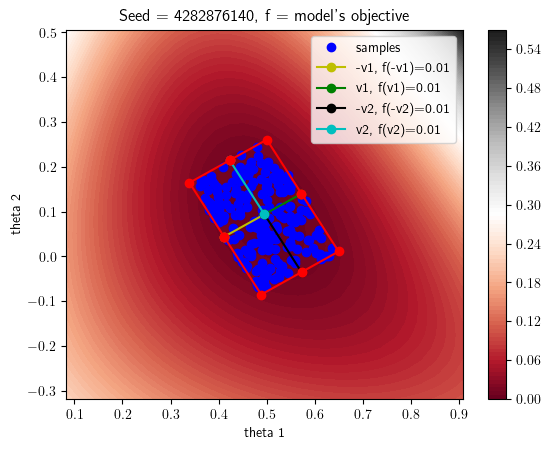
\includegraphics[width=0.55\textwidth]{./images/chapter4/ma2_region_1.png}
    \end{center}
  \caption[The acceptance region of a specific deterministic simulator.]{The acceptance region $S_i$ of a specific optimisation problem, that will contribute to the posterior.}
  \label{fig:ma2_5}
\end{figure}
\end{frame}

\begin{frame}
  \frametitle{ROMC - Training/Fitting part}
  \begin{algorithmic}[1]
    \Procedure{ROMC}{}
    \For{$i \gets 1 \textrm{ to } n_1$}
      \State $\mathbf{v}_i \sim p(\mathbf{v})$ \Comment{Draw nuisance variables}
      \State $f_i(\thetab)$ \Comment{Define deterministic simulator}
      \State $\thetab_i^* = \text{argmin}_{\thetab} |f_i(\thetab) - D|$ \Comment{Solve optimization problem}
      \If{$|f_i(\thetab) - D| > \epsilon$}
        \State Go to 2 \Comment{Filter solution}
      \EndIf
      \State Define the proposal area $\mathcal{\hat{S}}_i$ \Comment{Estimate proposal area}
    \EndFor
    \EndProcedure
  \end{algorithmic}

  \noindent\makebox[\linewidth]{\rule{\paperwidth}{0.4pt}}
  Algorithmic view of the training part of ROMC
\end{frame}

\begin{frame}
  \frametitle{ROMC - Training part (Recap)}

  \begin{itemize}
  \item Target of Bayesian Inference
    \begin{itemize}
    \item infer the \textcolor{blue}{posterior distribution $p(\thetab|D)$}
    \end{itemize}
  \item ROMC proposal
    \end{itemize}
    \begin{equation}
      p(\thetab|D) \approx p(\thetab) \frac{1}{N} \sum_i \mathcal{S}_i(\thetab)
    \end{equation}

    \begin{itemize}
    \item where
      \begin{itemize}
      \item $\mathcal{S}_i(\thetab) = \frac{1}{V}$ if $|f_i(\thetab) - D| < \epsilon$, otherwise $0$
      \item $V$ is the volume of $\mathcal{S}_i(\thetab)$
      \end{itemize}
    \end{itemize}
  \noindent\makebox[\linewidth]{\rule{\paperwidth}{0.4pt}}
  ROMC approximation of the posterior distribution using only the simulator
\end{frame}

\begin{frame}
  \frametitle{ROMC - Prediction part}
  \begin{algorithmic}[1]
    \\\hrulefill
    \Procedure{ROMC}{}
    \For{$i \gets 1 \textrm{ to } n_1$}
        \For{$j \gets 1 \textrm{ to } n_2$}
        \State $\thetab_{ij} \sim q_i$, compute $w_{ij}$ \Comment{Sample}
      \EndFor
    \EndFor
    \State $E_{p(\thetab|D)}[h(\thetab)]$ \Comment{Estimate an expectation}
    \State $p_{d,\epsilon}(\thetab)$ \Comment{Evaluate the unnormalized posterior}
    \\\hrulefill
    \EndProcedure
  \end{algorithmic}
  \noindent\makebox[\linewidth]{\rule{\paperwidth}{0.4pt}}
  Algorithmic view of the prediction part of ROMC; how to sample from the posterior and
  estimate an expectation.

\end{frame}

\begin{frame}
  \frametitle{ROMC - Prediction part}
  \begin{itemize}
  \item Target of Bayesian Inference
    \begin{itemize}
    \item infer the \textcolor{blue}{predictive distribution $p(y|x,D)$}
    \end{itemize}
  \item ROMC proposal
    \begin{itemize}
    \item Sample from each samples from each acceptance region $(w_{ij}, \thetab_{ij})$
      \item Normalize them to sum to one $w_{ij} = \frac{1}{\sum_j w_{ij}}$
      \item $p(y|x, D) \approx \sum_i \sum_j w_{ij}f_i(\thetab, x)$
      \end{itemize}
    \end{itemize}
  \noindent\makebox[\linewidth]{\rule{\paperwidth}{0.4pt}}
  ROMC approximation of the predictive distribution using only the simulator

\end{frame}

\begin{frame}
  \frametitle{ROMC - Advantages}
  \begin{itemize}
  \item Efficient and Embarrassingly Parallel Framework for likelihood-free inference
  \item \alert{Efficient}, because it turns every random-generating
    process to a deterministic optimization problem \( \Rightarrow \)
    does not spend samples unreasonably
  \item \alert{Embarrassingly Parallel}, all optimisation processes
    can run in parallel \( \Rightarrow \) super-fast if many cores are accesible
  \item \alert{Framework}, because is a general recipe. The components
    that will be used depend on the user e.g. gradient-based optimizer
    or bayesian optimization
  \end{itemize}
  \noindent\makebox[\linewidth]{\rule{\paperwidth}{0.4pt}}
  ROMC is efficient and parallelizable.
\end{frame}

\subsection{Implementation at ELFI}
\begin{frame}
  \frametitle{Implementation at ELFI}
  \begin{itemize}
  \item Fully parallelizable and extendable implementation at ELFI
  \item \href{https://elfi.readthedocs.io/en/latest/}{https://elfi.readthedocs.io/en/latest/}
  \item Interactive jupyter notebooks with examples (google colab - no need for installing anything)
  \begin{itemize}
  \item \href{https://colab.research.google.com/drive/1lGRp0XrNfZ64NN0ASB_tYEKowXwlveDC}{Simple 1D example}
  \item \href{https://colab.research.google.com/drive/1Fof_WmCi1YizzSI_63aEsbLXsno5gSZ3}{Simple 2D example}
  \item \href{https://colab.research.google.com/drive/1nkdACQ370SSc0KB1bHv4sBRaxMlMqoNH}{Moving Average example}
  \item \href{https://colab.research.google.com/drive/1RzB-V1QueP1y1nyzv_VOqR1nVz3DUH3v}{Tutorial for extending the ROMC method with a Neural Network}
  \end{itemize}
  \item Paper about to be submited at JSS
  \end{itemize}
  \noindent\makebox[\linewidth]{\rule{\paperwidth}{0.4pt}}
  Feel-free to experiment with ROMC
\end{frame}


\subsection{Future Ideas}

\begin{frame}
  \begin{itemize}
  \item Find ways to make it efficient in high dimensional parametric
    space ( \(\approx 20 \) is high for LFI methods)
  \item Implement ROMC in a package with automatic differentiation, to
    see how it scales in higer-dimensions
  \item JAX a good candidate, provides novel way to freeze the seed
    without global side-effects
  \item Research for better (accurate and efficient) ways to estimate
    the regions \( \mathcal{S}_i \) in high-dimensions
  \end{itemize}
  \noindent\makebox[\linewidth]{\rule{\paperwidth}{0.4pt}}
  Stay alert, there will be updates!
\end{frame}